\subsection{Detailed list}
\label{subsect:Detailed list}
A \textit{visitor} should be able to:
\begin{description}
\item[[G1]] sign up into the system:
	\begin{description}
	\item[[D1]] every inserted e-mail must be unique;
	\newline
	\item[[R1]] the system checks if the e-mail inserted is real;
	\item[[R2]] a user cannot sign up with the same e-mail twice.
	\end{description}
\end{description}

\noindent A \textit{user} should be able to:
\begin{description}
\item[[G2]] log into the system:
	\begin{description}
	\item[[D1]] every inserted e-mail must be unique;
	\newline
	\item[[R3]] the e-mail and password inserted must be correct;
	\item[[R4]] incorrect credentials prevent the user from logging in.
	\end{description}
\item[[G3]] create an event specifying its location, date, starting and ending time:
	\begin{description}
	\item[[D2]] every event is related to a location;
	\item[[D3]] an event must happen in an existing place;
	\item[[D4]] an event to attend cannot be in the past;
	\item[[D5]] the starting time of an event is always specified;
	\item[[D6]] the ending time of an event is not mandatory;
	\newline
	\item[[R5]] a user must specify all mandatory fields to add the new event;
	\item[[R6]] the system reserves the specified time-slot for the event;
	\item[[R7]] the system warns the user if the inserted event overlaps with an already existing one;
	\item[[R8]] if the ending time of an event is not specified, the systems considers as ending time the hour of departure for the successive event;
	\item[[R9]] when an event is inserted after an event without a specified ending time, the ending time  of the first event is anticipated as stated in [R8].
	\end{description}
\item[[G4]] obtain the best travel path (according to his preferences) and the list of eventual feasible alternatives to reach a location:
	\begin{description}
	\item[[D7]] a person can travel only on one travel mean at once; 
	\item[[D8]] allowed travel means are cars, trains, metro, on foot, trams, bicycles, taxis, car sharing, bike sharing;
	\item[[D9]] every travel is programmed with a combination of one or more travel means;
	\newline
	\item[[R10]] every travel path proposed must be feasible in the available time (the interval between two consecutive events);
	\item[[R11]] if the travel involves two or more travel means, the starting location of the first proposed travel path and the ending location of the last proposed travel path must coincide respectively with the starting location and the ending location of the whole planned travel;
	\item[[R12]] the system does not consider paths that violate constraints on travel means defined by the user;
	\item[[R13]] the system checks user preferences to decide which feasible travel path is the best;
	\item[[R14]] the system warns the user if it is not possible to arrive at an event location before its starting time;
	\item[[R15]] appropriate travel means must be suggested according to the type of event that they are related to; 
	\item[[R16]] if a strike occurs, the system will not consider travel means involved in it;
	\item[[R17]] if the weather forecasts rain or other adverse conditions, the system will not consider paths involving the bicycle.
	\end{description}
\item[[G5]] change the selected path with an alternative one:
	\begin{description}
	\item[[D7]] a person can travel only on one travel mean at once; 
	\item[[D8]] allowed travel means are cars, trains, metro, on foot, trams, bicycles, taxis, car sharing, bike sharing;
	\item[[D9]] every travel is programmed with a combination of one or more travel means;
	\newline
	\item[[R18]] the system must show to the user all possibilities to reach a location in according with the requirements of [[G4]];
	\item[[R19]] alternative feasible travel paths must not generate overlappings with other events of the schedule.
	\end{description}
\item[[G6]] obtain a daily schedule that allows him to attend every event in program:
	\begin{description}
	\item[[D10]] a person can be only in one place at once;
	\newline
	\item[[R20]] the combination of the travel paths proposed for the day must be feasible in the allotted time;
	\item[[R21]] if there are multiple events at the same time the system will propose in the schedule only the first event added.
	\item[[R22]] if the user forces into the schedule an event that overlaps with events already present in the schedule, these are removed from the schedule.
	\end{description}
\item[[G7]] apply constraints on travel means:
	\begin{description}
	\item[[D7]] a person can travel only on one travel mean at once; 
	\item[[D8]] allowed travel means are cars, trains, metro, on foot, trams, bicycles, taxis, car sharing, bike sharing;	
	\item[[D9]] every travel is programmed with a combination of one or more travel means;
	\newline
	\item[[R23]] the system requires minimum and maximum length allowed for a path to impose a constraint on a travel mean;
	\item[[R24]] the system requires an interval of time allowed to impose a constraint on a travel mean;
	\item[[R25]] the system does not consider solutions that violate constraints.
	\end{description}
\item[[G8]] deactivate one or more travel means:
	\begin{description}
	\item[[D7]] a person can travel only on one travel mean at once; 
	\item[[D8]] allowed travel means are cars, trains, metro, on foot, trams, bicycles, taxis, car sharing, bike sharing;	
	\item[[D9]] every travel is programmed with a combination of one or more travel means;
	\newline
	\item[[R26]] the system allows the user to specify one or more travel means that cannot be used;
	\item[[R27]] the system does not consider solutions that include deactivated travel means.
	\end{description}
\item[[G9]] select combinations of transportation means that minimize carbon footprint:
	\begin{description}
	\item[[D11]] every travel mean is related to information about its average carbon footprints;
	\newline
	\item[[R28]] for each travel path, the system estimates its carbon footprint produced.
	\end{description}
\item[[G10]] reserve time for lunch or break events:
	\begin{description}
	\item[[D12]] a flexible time-slot can have a daily or periodical validity;
	\item[[D13]] a flexible time-slot has a minimum amount of time that must be reserved;
	\newline
	\item[[R29]] the system allows the user to specify a flexible interval and a minimum amount of time to schedule a break;
	\item[[R30]] if there is enough time for a break, the system reserves it within the specified flexible interval;
	\item[[R31]] if there is not enough time into the flexible interval specified, a warning is thrown.
	\end{description}
\item[[G11.1]] arrange trips (buy needed tickets):
	\begin{description}
	\item[[D14]] a ticket is required to use a public transport;
	\item[[D15]] a ticket may have a daily validity or a different periodicity;
	\item[[D16]] a user can own day/week/season passes;
	\newline
	\item[[R32]] the system allows the user to specify all the ticket he already owns;
	\item[[R33]] the system shows to the user if he already holds a ticket for a proposed travel;
	\item[[R34]] the system allows the user to buy public transportation tickets according to proposed travels;
	\item[[R35]] the system provides information about time of departure and arrival of the proposed travels.
	\end{description}
\item[[G11.2]] arrange trips (find available sharing vehicles):
	\begin{description}
	\item[[D17]] a payment is required to use a sharing vehicle;
	\newline
	\item[[R36]] the system shows to the user where sharing vehicles are located;
	\item[[R37]] the system provides information about travel time with shared vehicles.
	\end{description}
\end{description}

\subsection{Scenarios}
\label{subsect:Scenarios}
	\subsubsection{Scenario 1}
		Oscar is a businessman who travels a lot and he would like to organize his travels quickly and precisely. A friend advises him to try Travlendar+. Oscar enters the Travlendar+ website and loads the registration page by clicking on the 'signup' button, he fills all the mandatory fields and then he receives a confirmation email and he clicks on the confirmation link inside.
Then Oscar logs in and starts using Travlendar+.
	\subsubsection{Scenario 2}
		Nigel lives in Milan and tomorrow he’s going to have an appointment in Lecco, so he has to decide how to reach his appointment location; Nigel accesses the login page from his personal computer by using his browser, fills the username and password fields, clicks on the 'confirm' button and logs in. After he clicks on the dedicated button that adds a new event, he fills all the requested fields, setting the event type as 'work meeting' in order to obtain proper suggested travel means, then he confirms the event creation. On the next day, Nigel travels to Lecco, following the travel schedule proposed by his Travlendar+ app, reaching his appointment right on time.
	\subsubsection{Scenario 3}
		Jasper inserts an event into his Travlendar+ calendar, but the location inserted is too far away from his previous event, therefore a feasible path to reach the location of the next event is not available in the allotted time. Jasper is notified by a warning that he will not be able to reach his appointment in time.	
	\subsubsection{Scenario 4}
		Ophelia inserts a new event into his Travlendar+ calendar, but that event overlaps with another already existing event. Ophelia is notified by her app and the system asks Ophelia to choose which one of the overlapping events she wants to attend. She chooses the last event inserted, then she reads the travel means proposed to respect her new time schedule.
	\subsubsection{Scenario 5}
		Henrietta wants to personalize her Travlendar+ experience, so she clicks on the ‘menu’ icon and then the voice ‘preferences’. She selects her preferred travel means, she chooses to always obtain the fastest path and then, since she walks with a limp, she inserts a maximum walking distance of 500 meters. Before clicking on the 'confirm' button, she sees a polluting truck outside her window, so she decides to always follow travel paths that minimize her carbon footprint. She selects the relative option in her preferences. Finally she clicks on the ‘confirm’ button and she observes that her suggested travels have changed according to her new preferences.
	\subsubsection{Scenario 6}
		Arthur can\textsc{\char13}t concentrate on his work if he doesn't eat his lunch between 12.00 and 13.00. He also needs at least 25 minutes to consume a proper lunch.
For this reason Arthur inserts a flexible break event into his Travlendar+ calendar, in order to be sure that every day his app will reserve a time slot for his lunch.
A week later, Arthur inserts a new event whose travel overlaps with his flexible lunch event and his app notifies him. Arthur decides to ignore the warning, since he'll s going to eat during his travel.
	\subsubsection{Scenario 7}
		Gwendolyn looks at her Travlendar+ app and discovers that on the next day she has to travel first by train to Milan and then take a bike of MoBike’s sharing system in Milan. She clicks on the train travel slot in order to buy the proper ticket and the apps redirects her in the right Trenord’s online shop webpage. When she is about to buy the ticket she suddenly remembers that she has a weekly Trenord pass, therefore she cancels the transaction and, in order to avoid making the same mistake twice, she adds her pass information into her Travlendar+ app. The next day Gwendolyn takes the train to Milan and when she arrives she opens her Travlendar+ app in order to find the nearest bike of MoBike’s. Gwendoline arrives in time at her appointment.
	\subsubsection{Scenario 8}
		Harvey has to reach an appointment near his home next week. He adds an event in his Travlendar+ calendar. He observes that the app suggests him to use a bike to reach the location of this event. The day before his appointment the weather forecasts rain for the successive day, so Harvey is notified by his app that, due to the forecast, he should avoid taking the bike, suggesting instead to reach his appointment by car.
	\subsubsection{Scenario 9}
		Sara inserts an event in her Travlendar+ calendar, then she looks at the proposed travel path. Since she did not like the proposed travel, she clicks on the proposed path and selects another feasible alternative. The next day Sara travels according to the travel path she likes more.	
	
\subsection{Use case descriptions}
\label{subsect:Use case descriptions}

	\subsubsection{[UC1] Registration}
		\begin{table}[H]
	\begin{center}
		\begin{tabular}{ | p{0.3\textwidth} | p{0.7\textwidth} | }
		\hline
		Participating actors & Generic visitor\\
		\hline
		Entry Condition & There are no entry conditions.\\
		\hline
		Event Flow & 
			\begin{enumerate}
				\item The visitor clicks on the “Register” button displayed onto the homepage;
				\item The visitor fills all the mandatory fields shown required by the system including his email, his password (twice) and a captcha;
				\item The visitor clicks on “Confirm” button;
				\item The visitor receives a confirmation email and clicks on the confirmation link;
				\item The system saves all user data inserted.
			\end{enumerate} \\
		\hline
		Exit Condition & The visitor’s registration is completed successfully, so the visitor is registered as an user of Travlendar+ and he can log in into the system as a registered user. \\
		\hline
		Exception & If:
				\begin{itemize}
   					\item The visitor insert an email already connected to an existing account;
   					\item Insert invalid infos into in some mandatory field;
   					\item Leave empty a mandatory field;
   				\end{itemize}
   		Then the system will request the visitor to complete/ revise all uncorrected field, highlighting them.
if the visitor doesn’t activate the account, after a month the activation link will expire and all user data will be deleted.\\ 
		\hline
		\end{tabular}
	\end{center}
	\caption{registration use-case}
\end{table}
		
	\subsubsection{[UC2] Login}
		\begin{table}[H]
	\begin{center}
		\begin{tabular}{ | p{0.3\textwidth} | p{0.7\textwidth} | }
		\hline
		Participating actors & Unauthenticated User\\
		\hline
		Entry Condition & There are no entry conditions.\\
		\hline
		Event Flow & 
			\begin{enumerate}
				\item The visitor clicks on the 'Login' button displayed on the homepage;
				\item The visitor inserts the email and the password previously used for registration;
				\item The visitor clicks on 'Confirm' button;
				\item The system redirect the user to the main view of Travlendar+.
			\end{enumerate} \\
		\hline
		Exit Condition & The Visitor’s login is completed successfully, so the visitor can use all the Travlendar+ functions. \\
		\hline
		Exception & If:
				\begin{itemize}
   					\item The email inserted is not one of the emails previously used by an user to sign up;
   					\item The password inserted by the visitor is not the one associated with the email inserted;
   					\item At least one of the field is left empty;
   				\end{itemize}
   		Then the system will notify the visitor to complete/ revise all uncorrected field, highlighting them.\\ 
		\hline
		\end{tabular}
	\end{center}
\end{table}
		
	\subsubsection{[UC3] View calendar}
		\begin{table}[H]
	\begin{center}
		\begin{tabular}{ | p{0.3\textwidth} | p{0.7\textwidth} | }
		\hline
		Participating actors & User\\
		\hline
		Entry Condition & The user must be logged in Travlendar+.\\
		\hline
		Event Flow & 
			\begin{enumerate}
				\item The user clicks on the calendar button;
				\item The system shows a calendar including all inserted events, and the travel paths related.
			\end{enumerate} \\
		\hline
		Exit Condition & The system let the user check his calendar. \\
		\hline
		Exception & There are no exceptions.\\ 
		\hline
		\end{tabular}
	\end{center}
\end{table}
		
	\subsubsection{[UC4] Create event}
		\begin{table}[H]
	\begin{center}
		\begin{tabular}{ | p{0.3\textwidth} | p{0.7\textwidth} | }
		\hline
		Participating actors & User.\\
		\hline
		Entry Condition & The user must be registered and logged in Travlendar+\\
		\hline
		Event Flow & 
			\begin{enumerate}
				\item The user clicks on the dedicated button to add a new event;
				\item The user inserts all the info related to the event: date, starting time, ending time, location, name of the event, type of event (predefined or personalized), description, location starting from to reach the event's location;
				\item The user confirms the creation of the event;
				\item The system computes the best possible path according to the  user's preferences.
			\end{enumerate} \\
		\hline
		Exit Condition & The system redirects the user to the calendar and adds the travel time slot required to reach that event (comprehensive of travel description). \\
		\hline
		Exception & If the inserted event overlaps with one or more previously added events (the travel is also considered in the eventual overlap), then the user is notified with a warning message and the overlapping event is not considered in the user travel planning schedule (but it remains saved in the calendar). The user has to choose which one of the overlapped events does he want to attend.\\ 
		\hline
		\end{tabular}
	\end{center}
	\caption{Create event use-case}
\end{table}
		
	\subsubsection{[UC5] Create personalized event profiles}
		\begin{table}[H]
	\begin{center}
		\begin{tabular}{ | p{0.3\textwidth} | p{0.7\textwidth} | }
		\hline
		Participating actors & User.\\
		\hline
		Entry Condition & The user must be registered and logged in Travlendar+.\\
		\hline
		Event Flow & 
			\begin{enumerate}
				\item The user opens the preferences menu;
				\item The system shows the default type of event;
				\item The user selects the tab "Create personalized type of event";
				\item The system shows a page containing a text field to fill;
				\item The user inserts the name of the personalized type of event that he wants to create;
				\item The user inserts the constraints on travel means related to that type of event;
				\item The user clicks on the "Save" button;
				\item The system adds the new type of events to those already existing.

			\end{enumerate} \\
		\hline
		Exit Condition & The user has successfully added a new personalized type of event in the system.\\
		\hline
		Exception & If the user exits the page without clicking the "Save" button, then the system will not save the new personalized type of event created by the user.\\ 
		\hline
		\end{tabular}
	\end{center}
	\caption{Create personalized event profiles use-case}
\end{table}
		
	\subsubsection{[UC6] Define flexible breaks}
		\begin{table}[H]
	\begin{center}
		\begin{tabular}{ | p{0.3\textwidth} | p{0.7\textwidth} | }
		\hline
		Participating actors & User.\\
		\hline
		Entry Condition & The user must be registered and logged in Travlendar+.\\
		\hline
		Event Flow & 
			\begin{enumerate}
				\item The user clicks on the dedicated button to add breaks into the schedule;
				\item The user inserts a flexible period of time (specifying starting and ending time) that will contain the break, along with the minimum amount of time that will be dedicated to it;
				\item The user also specifies the periodicity of the break (daily, weekly, monthly or until a specified date) or if it refers only to certain days of the week (until a specified date);
				\item The user presses the "Save" button. 
			\end{enumerate} \\
		\hline
		Exit Condition &  The system notifies the user that the info inserted about breaks are correctly saved.\\
		\hline
		Exception & If it is not possible to dedicate the allotted time to the breaks because of previously added events, than the system asks the user to change the length of the break.
\\ 
		\hline
		\end{tabular}
	\end{center}
	\caption{Define flexible breaks use-case}
\end{table}	
		
	\subsubsection{[UC7] Arrange trips}
		\begin{table}[H]
	\begin{center}
		\begin{tabular}{ | p{0.3\textwidth} | p{0.7\textwidth} | }
		\hline
		Participating actors &  User, Transport service provider\\
		\hline
		Entry Condition & The user must be logged in Travlendar+.\\
		\hline
		Event Flow & 
			\begin{enumerate}
				\item The user opens his calendar
				\item The user clicks on the trip he want to arrange;
				\item The system shows all tickets to be buyed and the tickets already bought;
				\item The user clicks on the ticket he want to buy.
				\item The system redirect the user to the right website (of the right Transport service provider) in order to buy the tickets.
			\end{enumerate} \\
		\hline
		Exit Condition & The user has successfully arranged his travel. \\
		\hline
		Exception & There are no exceptions. \\ 
		\hline
		\end{tabular}
	\end{center}
	\caption{Arrange trips use-case}
\end{table}	
		
	\subsubsection{[UC8] Locate the nearest sharing vehicle}
		\begin{table}[H]
	\begin{center}
		\begin{tabular}{ | p{0.3\textwidth} | p{0.7\textwidth} | }
		\hline
		Participating actors &  User, Transport service provider\\
		\hline
		Entry Condition & The user has opened the arrange trip tab and is about to travel.\\
		\hline
		Event Flow & 
			\begin{enumerate}
				\item The user open the map;
				\item The system shows in the map the nearest vehicle of car sharing according to the chosen path and the infos provided by the transport service provider;
			\end{enumerate} \\
		\hline
		Exit Condition & The user take and use the suggested vehicle. \\
		\hline
		Exception &
				\begin{itemize}
   					\item If no near vehicle is found the system re-compute another path and show it to the user;
   					\item if the user take a shared vehicle, but not the suggested one nothing happen, just as he has taken the suggested vehicle;
   				\end{itemize} \\ 
		\hline
		\end{tabular}
	\end{center}
\end{table}	
		
	\subsubsection{[UC9] Add ticket possessed}
		\begin{table}[H]
	\begin{center}
		\begin{tabular}{ | p{0.3\textwidth} | p{0.7\textwidth} | }
		\hline
		Participating actors & User\\
		\hline
		Entry Condition & The user has opened the arrange trip tab.\\
		\hline
		Event Flow & 
			\begin{enumerate}
				\item The user selects the tab 'my tickets';
				\item The system show a page containing all the tickets and passes possessed by the user;
				\item The user clicks on the 'add ticket' button;
				\item The system show a page containing fields to fill;
				\item The user inserts info regarding the ticket/pass possessed;
				\item The user clicks on the 'save' button;
				\item The system adds the ticket/pass to those already present in the user account.
			\end{enumerate} \\
		\hline
		Exit Condition & The user has successfully inserted his ticket/pass in the system.\\
		\hline
		Exception & If the user exits the page without clicking the “save” button, then the system will not save the ticket added by the user.\\ 
		\hline
		\end{tabular}
	\end{center}
	\caption{Add ticket possessed use-case}
\end{table}	
	
	\subsubsection{[UC10] Obtain feasible travel paths}
		\begin{table}[H]
	\begin{center}
		\begin{tabular}{ | p{0.3\textwidth} | p{0.7\textwidth} | }
		\hline
		Participating actors & User, Google Maps APIs.\\
		\hline
		Entry Condition & The user must be registered and logged in Travlendar+.\\
		\hline
		Event Flow & 
			\begin{enumerate}
				\item The user opens the "Calendar" tab;
				\item The user selects a day in the calendar;
				\item The system shows the proposed feasible paths (shown as travel events) between the events;
				\item If the user wants to select an alternative travel path, he can clicks on the travel event in order to choose among the proposed feasible alternatives.
			\end{enumerate} \\
		\hline
		Exit Condition & The user has seen the possible travel paths that can be used to reach his meetings.\\
		\hline
		Exception & If no feasible travel path exists between two events, the system shows a warning in the calendar.\\ 
		\hline
		\end{tabular}
	\end{center}
	\caption{Obtain feasible travel paths use-case}
\end{table}	
	
	\subsubsection{[UC11] Choose between overlapping events}
		\begin{table}[H]
	\begin{center}
		\begin{tabular}{ | p{0.3\textwidth} | p{0.7\textwidth} | }
		\hline
		Participating actors & User\\
		\hline
		Entry Condition & The user must be logged in Travlendar+, at least two events are overlapped.\\
		\hline
		Event Flow & 
			\begin{enumerate}
				\item The user clicks on the calendar button;
				\item The system shows a calendar including all inserted events, and the travel paths related, the overlapping events are displayed in a separate way in respect to the actual day schedule;
				\item The user drag the chosen overlapping event into his day schedule;
				\item The system remove the precedent event (in conflict) and put it into the overlapping event list;
				\item The system shows the new day schedule, with updated travel paths.
			\end{enumerate} \\
		\hline
		Exit Condition & The system let the user check his calendar. \\
		\hline
		Exception & There are no exceptions.\\ 
		\hline
		\end{tabular}
	\end{center}
	\caption{Choose between overlapping events use-case}
\end{table}
		
	\subsubsection{[UC12] Edit event}
		\begin{table}[H]
	\begin{center}
		\begin{tabular}{ | p{0.3\textwidth} | p{0.7\textwidth} | }
		\hline
		Participating actors &  User.\\
		\hline
		Entry Condition & The user must be registered and logged in Travlendar+, at least one event must have been added.\\
		\hline
		Event Flow & 
			\begin{enumerate}
				\item The user clicks on a specific day;
				\item The user selects the edit option on the event he wants to modify;
				\item The system shows the fields where the user can change the information previously inserted;
				\item The user clicks on the confirm button;
				\item The system calculates the new travel according to the specifications of the user. The modified event remains in the schedule if it doesn’t overlap with another event.
			\end{enumerate} \\
		\hline
		Exit Condition & The system shows the new daily schedule, eventually with updated travel paths. \\
		\hline
		Exception & The user edits the location or the starting/ending time of the event in a way that attend to event is no more feasible. The user is notified with a warning message, the event is removed from the schedule.\\ 
		\hline
		\end{tabular}
	\end{center}
	\caption{Edit event use-case}
\end{table}
		
	\subsubsection{[UC13] Delete event}
		\begin{table}[H]
	\begin{center}
		\begin{tabular}{ | p{0.3\textwidth} | p{0.7\textwidth} | }
		\hline
		Participating actors &  User.\\
		\hline
		Entry Condition & The user must be registered and logged in Travlendar+, at least one event must have been added.\\
		\hline
		Event Flow & 
			\begin{enumerate}
				\item The user clicks on a specific day;
				\item The user selects the delete option on the event he wants to delete;
				\item The user clicks on the confirm button;
				\item If an overlapping event becomes feasible, the system calculates the travel and the event is added to the schedule.
			\end{enumerate} \\
		\hline
		Exit Condition & The system shows the new daily schedule, eventually with updated travel paths. \\
		\hline
		Exception & There are no exceptions.\\ 
		\hline
		\end{tabular}
	\end{center}
	\caption{Delete event use-case}
\end{table}
		
	\subsubsection{[UC14] Edit personalized event profiles}
		\begin{table}[H]
	\begin{center}
		\begin{tabular}{ | p{0.3\textwidth} | p{0.7\textwidth} | }
		\hline
		Participating actors &  User.\\
		\hline
		Entry Condition & The user must be registered and logged in Travlendar+, at least one type of event must have been added.\\
		\hline
		Event Flow & 
			\begin{enumerate}
				\item The user opens his preferences;
				\item The user selects the "Edit" button on the type of event he wants to modify;
				\item The system shows the settings associated to the type that the user wants to edit;
				\item The user can add, edit or delete single constraints;
				\item The user clicks on the "Confirm" button;
				\item If there is at least one event related to that type of event, the system asks to the user if he wants to apply changes on preferences to the existing events of that type. 
			\end{enumerate} \\
		\hline
		Exit Condition & The system saves the new set of constraints for the type of event modified and, eventually, updates the related events. \\
		\hline
		Exception & If an event is no more a feasible one, the system behaves like it is an exception for edit event.\\ 
		\hline
		\end{tabular}
	\end{center}
	\caption{Edit type of event use-case}
\end{table}
		
	\subsubsection{[UC15] Delete personalized event profiles}
		\begin{table}[H]
	\begin{center}
		\begin{tabular}{ | p{0.3\textwidth} | p{0.7\textwidth} | }
		\hline
		Participating actors &  User.\\
		\hline
		Entry Condition & The user must be registered and logged in Travlendar+, at least one type of event must have been added.\\
		\hline
		Event Flow & 
			\begin{enumerate}
				\item The user opens his preferences;
				\item The user selects the "Delete" option on the type of event he wants to delete;
				\item The user clicks on the "Confirm" button;
				\item If there is at least one event related to that type of event, the system asks the user if he wants to maintain the old preferences for the existing events of that type. 
			\end{enumerate} \\
		\hline
		Exit Condition & The system deletes that type of event from the preferences and, eventually, removes constraints from the related events. \\
		\hline
		Exception & There are no exceptions.\\ 
		\hline
		\end{tabular}
	\end{center}
	\caption{Delete type of event use-case}
\end{table}
		
\subsection{Use case diagrams}
\label{subsect:Use case diagrams}
	\subsubsection{Visitors}
		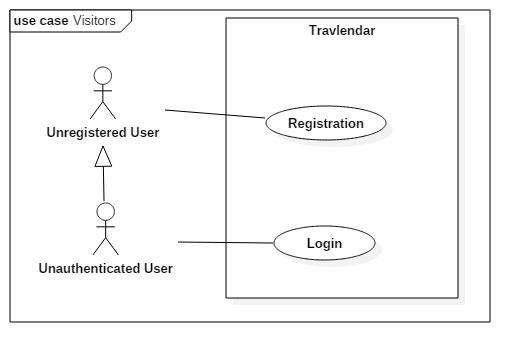
\includegraphics[scale=0.7]{Visitors.png}
	\subsubsection{User}
		\noindent\makebox[\textwidth]{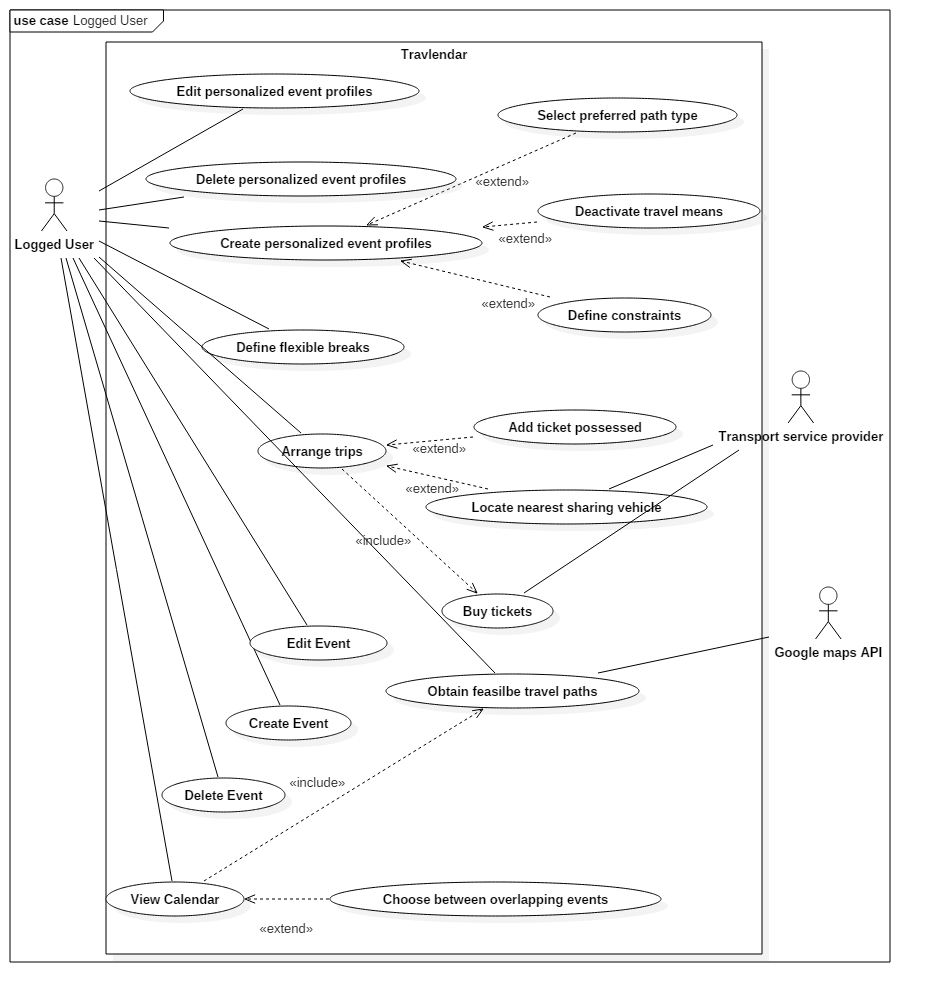
\includegraphics[width=\paperwidth,height=\paperheight,keepaspectratio]{LoggedUser.png}}
		
\subsection{Sequence diagrams}
\label{subsect:Sequence diagrams}
	\subsubsection{Login}
		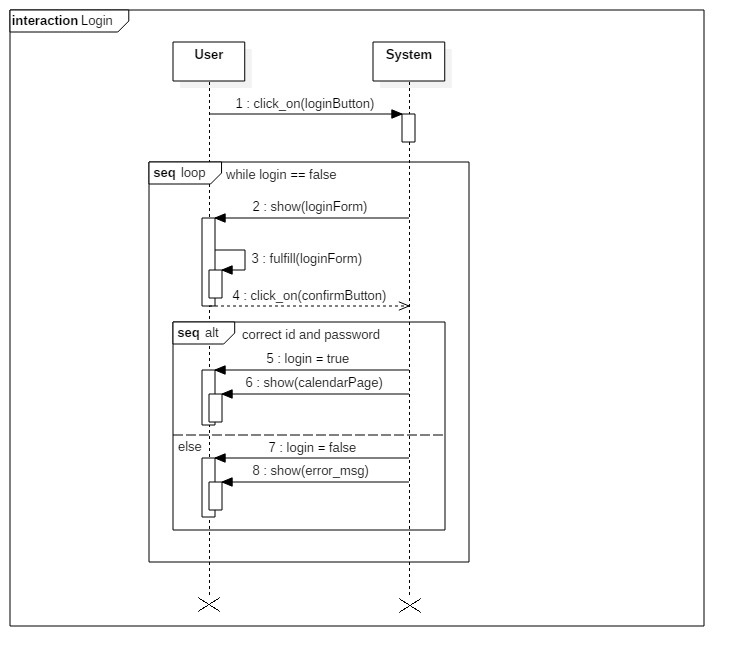
\includegraphics[scale=0.43]{sequence_diagrams/login.jpg}
	\subsubsection{Create event}
		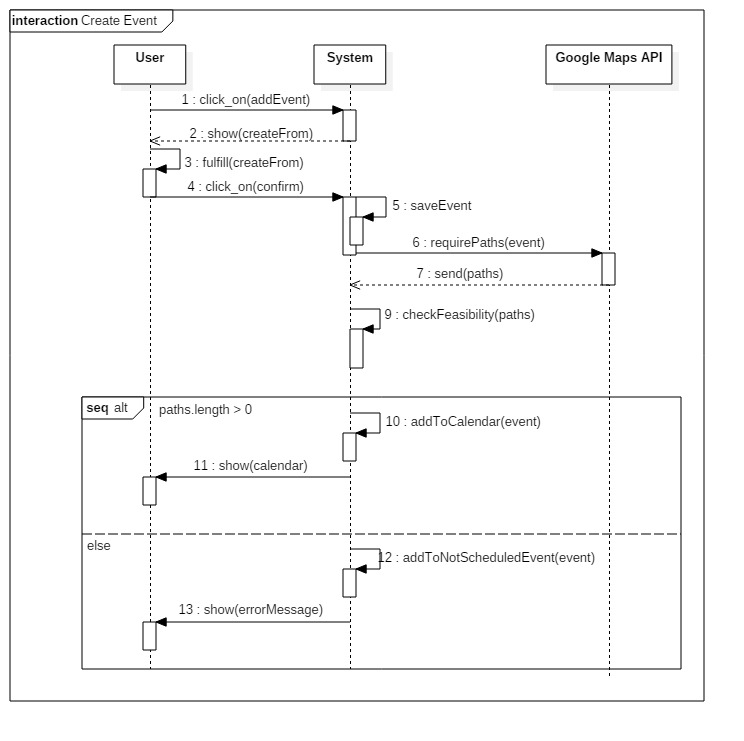
\includegraphics[scale=0.43]{sequence_diagrams/create_event.jpg}
	\subsubsection{Arrange trip}
		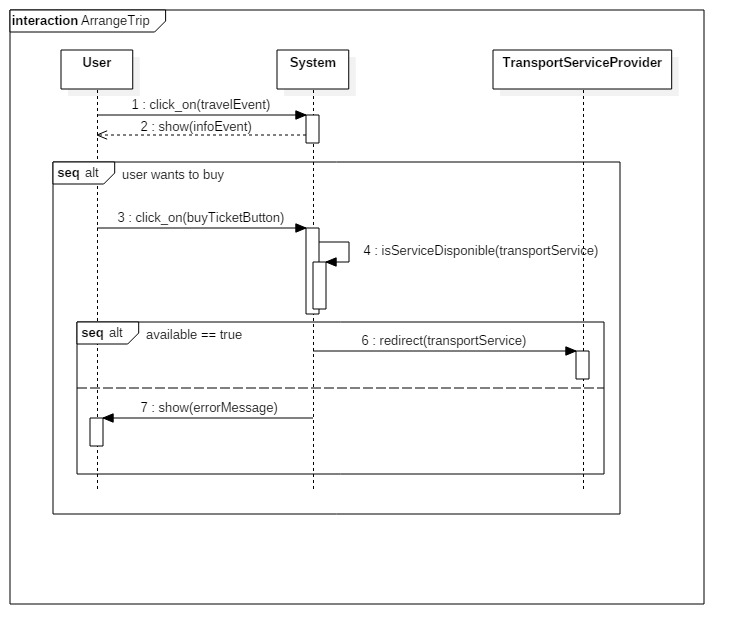
\includegraphics[scale=0.43]{sequence_diagrams/arrange_trip.jpg}
	\subsubsection{Obtain feasible paths}
		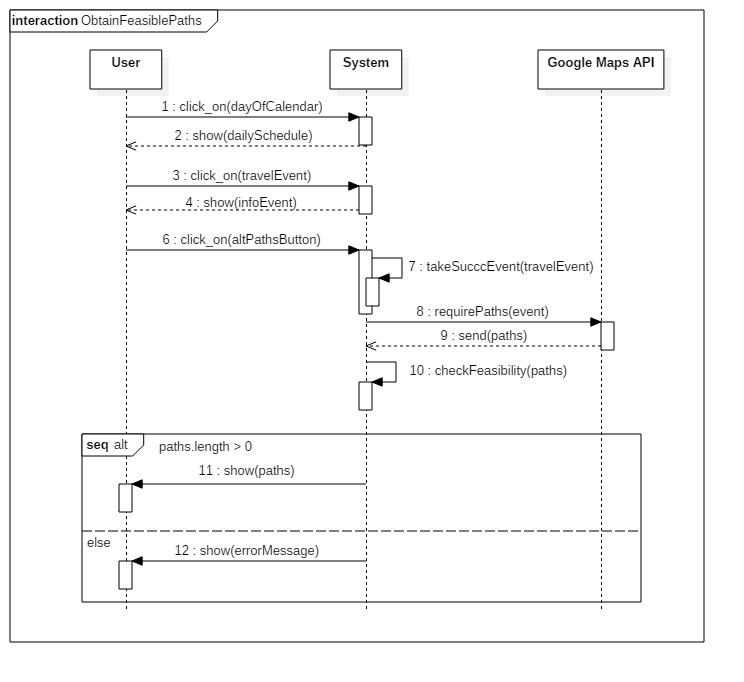
\includegraphics[scale=0.43]{sequence_diagrams/obtain_feasible_paths.jpg}
	\subsubsection{Choose between overlapping events}
		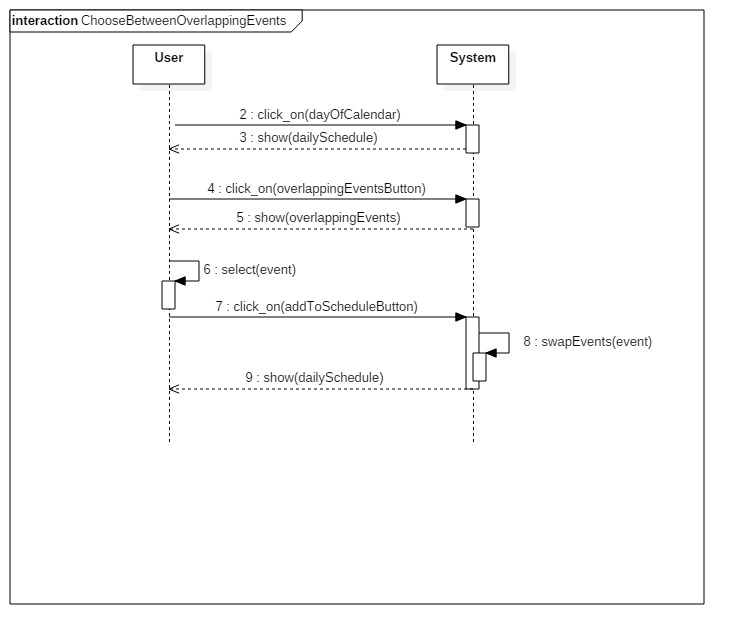
\includegraphics[scale=0.43]{sequence_diagrams/choose_between_overlapping_events.jpg}